\documentclass[25pt, colspace=1in, blockverticalspace=.2in]{tikzposter}
\usepackage[T1]{fontenc}
\tikzposterlatexaffectionproofoff

\geometry{paperwidth=48in,paperheight=36in}
\makeatletter
\setlength{\TP@visibletextwidth}{\textwidth-2\TP@innermargin}
\setlength{\TP@visibletextheight}{\textheight-2\TP@innermargin}
\makeatother

%\usepackage{xspace,amsmath,amsfonts,amssymb,hyperref,multirow,mathtools}
%\usepackage{biblatex}
%\usepackage{tkz-euclide}
%\usepackage{algpseudocode, algorithmicx}
%\usepackage{blkarray}
\usepackage[shortlabels]{enumitem}
\usepackage{lipsum}
\usepackage{varwidth, parskip}
\usepackage{booktabs}

\usetikzlibrary{positioning}
\usepackage[RPvoltages]{circuitikz}
\ctikzset{logic ports=ieee,logic ports/scale=1.5}
%\usetikzlibrary{shapes.geometric}
%\usetikzlibrary{intersections}
%\usetkzobj{all}

\newlength\linewidthscale
\setlength\linewidthscale{2.54pt}

\tikzset{
	 ultra thin/.style = {line width=0.1\linewidthscale},
	  very thin/.style = {line width=0.2\linewidthscale},
	       thin/.style = {line width=0.4\linewidthscale},
	      thick/.style = {line width=0.8\linewidthscale},
	 very thick/.style = {line width=1.2\linewidthscale},
	ultra thick/.style = {line width=1.6\linewidthscale}
}


\title{Mobile Cryptographic Coprocessor for Privacy-Preserving Two-Party Computation}
\author{Gabriel Kulp, mentored by Dr. Mike Rosulek}
\institute{Oregon State University School of Electrical Engineering and Computer Science}

\usetheme{Simple}
\usetitlestyle{Filled}

\definecolor{titlebgcolor}{HTML}{D73F09}
\definecolor{blocktitlefgcolor}{HTML}{D73F09}

%\def\HyperFirstAtBeginDocument#1{#1}
\begin{document}

\maketitle
\path (\titleposleft,\titleposbottom) ++(+1cm,5mm) node[inner sep=0pt,above right] {
\includegraphics[height=0.45\titlepostop-0.45\titleposbottom]{osu-logo.pdf}};
\path (\titleposright,\titleposbottom) ++(-1cm,5mm) node[inner sep=0pt,above left] {
\includegraphics[height=0.45\titlepostop-0.45\titleposbottom]{logo-white.pdf}};

%% To measure how wide it should be on the my screen.
%\draw[thick] (0, 0) to (344mm,0);

\begin{columns}


\column{0.33} % left column


\block{Abstract}{
	Multi-party computation (MPC) is a cryptographic protocol that allows parties to learn the output of some function of their private inputs without trusting a third party to perform the computation. This is usually done at a large scale between data centers, with little emphasis on individuals' devices or mobile hardware. In this project, I present a proof-of-concept implementation of two-party computation on a commodity smartphone paired with a low-power field-programmable gate array (FPGA). I compare the performance and power consumption of the system between a software-only setup and a setup with the FPGA co-processor used for acceleration. I find a calculated $260\times$ speed improvement assuming a saturated serial connection, and no significant difference in battery life.
}

\block{Boolean Circuits}{
	\begin{center}
	\begin{tikzpicture}[scale=1.7, every node/.style={transform shape}, thick]
		\node[xor port] (xor)  at (0, 0){};
		\node[and port] (andA) at (5, 1.4){};
		\node[and port] (andB) at (5,-1.4){};
		\draw
			(andA.in 1)  -- ++(-8, 0)
			(andB.in 2)  -- ++(-8, 0)
			(xor.in 1)   -| ++(-1, 1.4) node [below right] {A}
			(xor.in 2)   -| ++(-1,-1.4) node [above right] {B}
			(andA.in 2)  -|   (xor.out) node [      right] {C}
			(andB.in 1)  -|   (xor.out)
			(andA.out) node [above] {D} -- ++(1, 0)
			(andB.out) node [above] {E} -- ++(1, 0);
	\end{tikzpicture}
	\end{center}

	\vspace{1cm}
	A Boolean circuit is a collection of logic gates connected together by wires. Each wire receives a label, with the computation's inputs assigned to the wires on the left. Each gate then compares the labels on its inputs to its lookup table to determine what label to assign to its output wire on the right. The contents of the lookup table determine how the gate behaves, like AND and XOR, to describe each gate as a boolean function.

	Boolean circuits are able to evaluate any mathematical expression, so a system (like mine) capable of processing wires and gates can perform any computation by just providing the desired circuit definition.
}

\block{Garbled Circuits}{
	\begin{center}
	\begin{tikzpicture}[
			scale=1.7, every node/.style={transform shape},
			clearbox/.style={rectangle, draw, very thick, minimum size=20mm},
			clearIO/.style={rectangle, thick, minimum size=18mm},
			garbledbox/.style={rectangle, draw, very thick, minimum size=20mm,align=center},
			garbledIO/.style={rectangle, thick, minimum size=18mm, align=center},
			->, >=stealth, line width=4mm,
			node distance=2.5cm,
		]
		\node[clearIO] (i) {Input};
		\node[clearbox,   right=of i,black!20!white] (c) {Circuit};
		\node[clearIO,    right=of c] (o)  {Output};
		\node[garbledbox, below=of c] (gc) {Garbled \\ Circuit};
		\node[garbledIO,  below=of i] (gi) {Garbled \\ Input};
		\node[garbledIO,  below=of o] (go) {Garbled \\ Output};
		
		\draw[dashed, black!20!white] (i) -- (c);
		\draw[dashed, black!20!white] (c) -- (o);
		\draw[red]  (i)  -- (gi);
		\draw[blue] (gi) -- (gc);
		\draw[blue] (gc) -- (go);
		\draw[red]  (go) -- (o);

		\node at ($(c)+(0,-1.85cm)$) [
			single arrow,
			top color=black!20!white, bottom color=red,
			minimum height=2.55cm, minimum width=25mm,
			inner sep=0mm, rotate=270,
			single arrow head extend=1mm
		] {};

	\end{tikzpicture}
	\end{center}

	\vspace{1cm}

	A Garbled Circuits protocol allows two parties to supply parts of the input to a Boolean circuit and together compute the output, but without sharing their input with the other party. Rather than following the dotted lines in the picture from input to output, one party (traditionally called Alice, shown here in red) ``garbles'' the circuit by applying some private transformation to it. She then works with the other party (traditionally called Bob) to convert their inputs into garbled inputs. Since Bob doesn't know the secret transformation, he's the one to evaluate the circuit, albeit blindly, following the blue arrows. Finally, Alice helps Bob transform the garbled output back into a normal output. In my setup, Bob has the FPGA and uses it to more efficiently perform the blind evaluation of the garbled circuit.

}


\column{0.34} % middle column
\block{Software Approach}{
\begin{description}
	\item[Algorithm ]
		There are several standard optimizations to garbling and evaluating circuits. I implemented Point-and-Permute, Free-XOR, and Garbled Row Reduction, but not Half Gates (the most recent improvement by my mentor, Dr.~Rosulek) or any gadget-wise optimizations. Implementing the remaining state-of-the-art optimization techniques would be a good candidate for future work, since they would further improve evaluation speed.
	\item[Scalability ]
		My implementation uses a scalable streaming approach, wherein the first line of the circuit definition file is interpreted, computed, and transmitted before the next line is even read. This contrasts with an in-memory approach which would read the entire file, perform all computations, then transmit all messages. This means that the size of the circuit is not a concern for the garbler, and the evaluator can simply pass off the network traffic to the FPGA as it comes in. Considering that real-world circuits can easily be larger than a typical consumer-oriented computer's memory, streaming is essential to feasibility.
	\item[Protocol ]
		I send the minimum amount of information for each gate. Since the type and ID are already provided in-order from the circuit definition, I send and receive \textit{only} the AND gate ciphertexts, without padding or metadata, between the garbler and evaluator. The evaluator has a copy of the circuit definition file and uses it to annotate the received ciphertexts before forwarding the complete set of instructions to the FPGA for processing. As soon as the smartphone (garbler) finishes sending data to the FPGA, it has the result ready to return.
\end{description}
}


\block{Hardware Approach}{
	\begin{description}
		\item[Scalability ]
			I used an event-based design inside the FPGA. For example, the memory controller emits a signal when it has finished fetching or storing a value. Right now the design uses on-chip SRAM, which significantly limits the size of circuit that can be safely evaluated. The event-based architecture would make it trivial to integrate a new memory controller for a larger bank of DRAM. Similarly, a faster AES implementation relying on more lookup tables would easily slot into the current design without worrying about tweaking timings or delays in other components.
		\item[Limitations ]
			My choice of FPGA development platform placed many restrictions on my implementation. For example, I only have room on the chip to provision a block capable of performing half of an AES round in a single clock cycle. On a larger FPGA, I would have enough room to fully unroll the algorithm's loops and perform all AES rounds in a single clock cycle. Similarly, I would have more options for fast inputs and outputs.
	\end{description}

	\vspace{2cm}
	\centering
	\begin{tikzpicture} [
			scale=1.3, every node/.style={transform shape},
			box/.style={rectangle, draw, ultra thick, fill=black!5!white},
			arrow/.style={ultra thick, <->, >=stealth},
			inner sep=7mm, align=center
		]
		\node at (0,7)  [box] (cloud) {Cloud (Garbler)};
		\node at (0,0)  [box] (phone) {Smartphone \\(Evaluator)};
		\node at (11,0) [box] (fpga) {FPGA};
		
		\draw [arrow] (cloud) -- (phone) node[midway, right] {Internet};
		\draw [arrow] (phone) -- (fpga)  node[midway, below] {USB};
	\end{tikzpicture}

	\vspace{1cm}
	\begin{varwidth}{.25\textwidth}
		System topology. \textit{I used my laptop on the local network as the garbler for simplicity, but the system could work with the same code running on a cloud server across the internet.}
	\end{varwidth}
}



\column{0.33} % right column


\block{FPGA Internals}{
	\begin{center}		
	\begin{tikzpicture}
		\node (image) {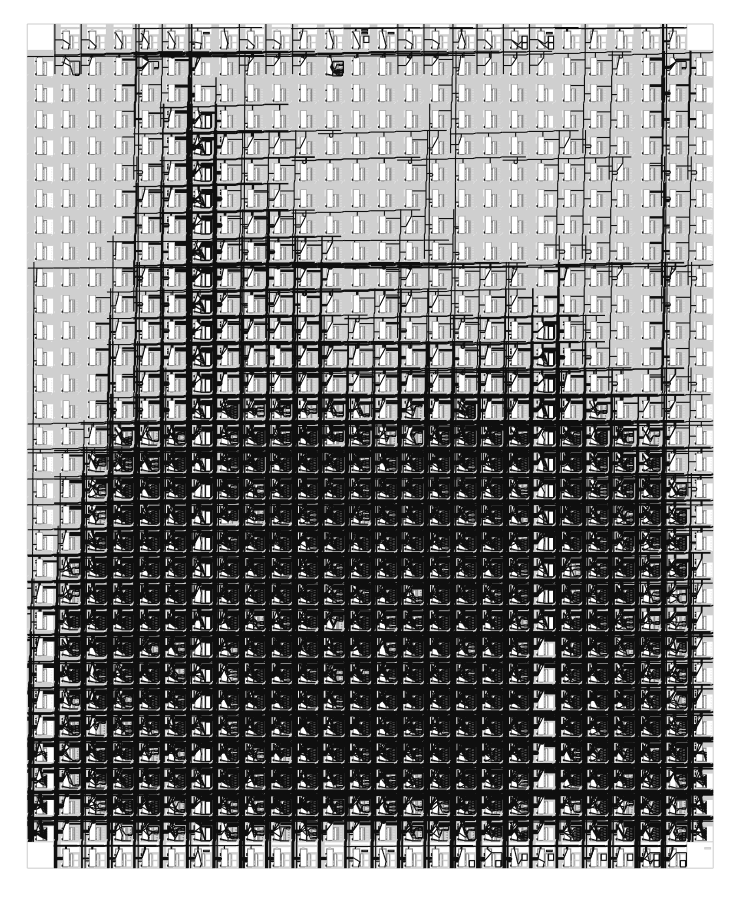
\includegraphics[width=.15\textwidth]{../figures/fabric-full.png}};
		\draw[white, fill] (3,0) circle(7mm);
		\draw[white, line width=4mm]
			(125:7.8) ++(17,0) coordinate(top)
			(-125:7.8)++(17,0) coordinate(bottom)
			(125:.5)  ++(3,0) -- (top)
			(-125:.5) ++(3,0) -- (bottom);
		\begin{scope}[even odd rule]
			%\draw[white, fill] (17,0) circle(8cm);
			\draw[black, ultra thick, fill=white] (17,0) circle(7.8cm);
			\clip (17,0) circle(7.5cm);
			\node (image) at (17,0) {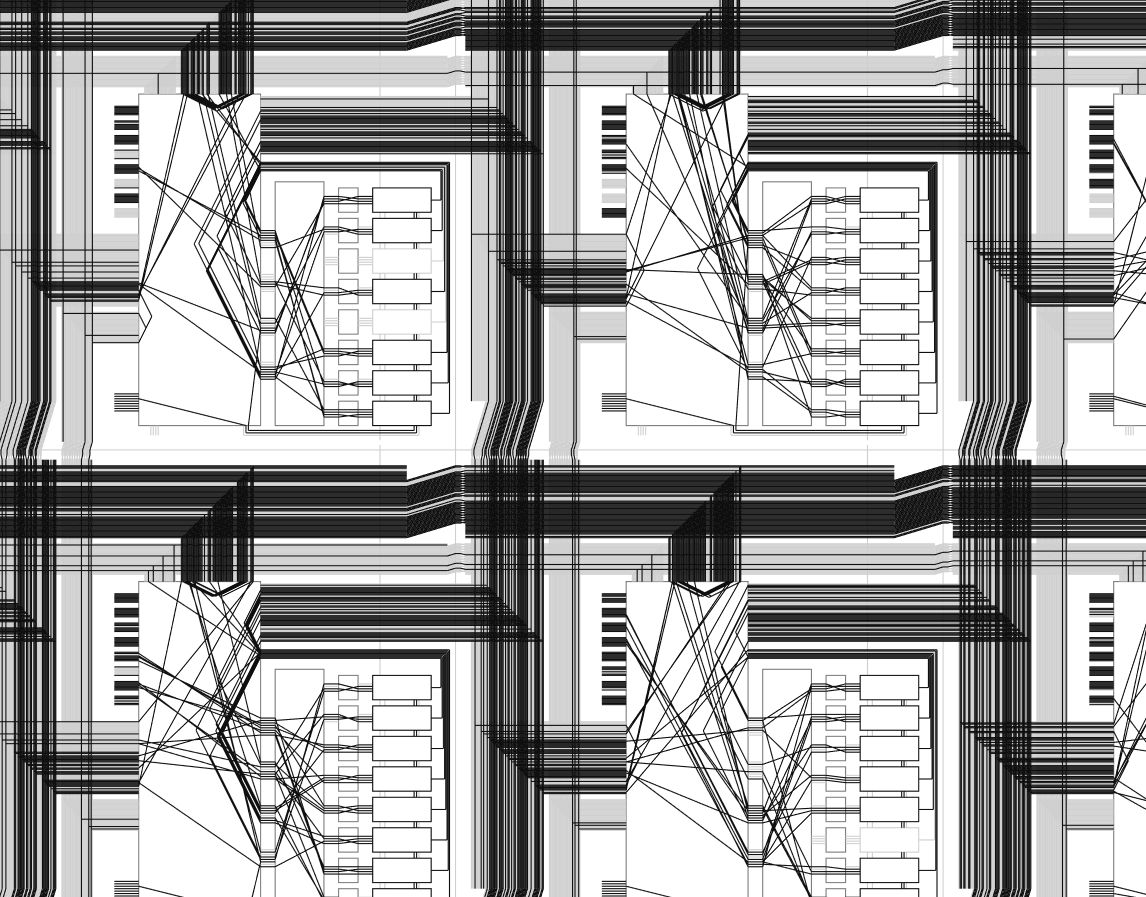
\includegraphics[height=15cm]{../figures/fabric-zoom.png}};
		\end{scope}
		\draw[black, ultra thick]
			(120:7.8) ++(17,0) coordinate(top)
			(-120:7.8)++(17,0) coordinate(bottom)
			(120:.5)  ++(3,0) -- (top)
			(-120:.5) ++(3,0) -- (bottom);
		\draw[black, ultra thick, fill=white] (3,0) circle(5mm);
		\draw(image.south)++(0,-4); % add some padding
	\end{tikzpicture}
	\begin{varwidth}{.25\textwidth}
		Place and route output of my hardware design. \textit{The black wires represent the allocated interconnects. The zoomed portion shows the reconfigurable internals of each logic cell.}
	\end{varwidth}
	\vspace{2cm}
	\end{center}

	FPGA stands for \textit{Field-Programmable Gate Array}. Running my coprocessor on an FPGA allows me to avoid the prohibitively expensive process of manufacturing a ``real'' single-purpose chip, while still letting me test on hardware instead of simulations alone. The \textit{gate array} part of the name means that the chip is made of a grid of general-purpose elements, shown in the zoomed-out view on the left above. Zooming in, you can see diagonal wires connecting the bus lines together inside some of these elements. The \textit{field-programmable} part of the name means that these connections can be reconfigured on-the-fly after the chip has been manufactured and shipped. I used this reprogramming capability to test each iteration of my design.
}

\block{Results}{
	With the FPGA fully utilized, the calculated \textbf{performance improvement is 260x} compared to a software-only system. In my setup, the connection between the FPGA and the smartphone was too slow to sustain this speed, and the real-world performance is 25\% slower than without the FPGA. Battery life was not significantly affected when using the FPGA.

	~

	For a benchmark, I performed a 64-bit floating point square root where each party supplies half of the representation of the number to take a square root of. While this is not a computation with much use in the real world, the actual computation has little bearing on the per-gate performance of the system. On average, evaluating a gate took 80 clock cycles and waiting for the next gate took 5000 cycles. In a fully-integrated system-on-chip, the connection speed between the smartphone's processor and the FPGA would be far above the bottleneck presented by the network speed.

	~

	In conclusion, MPC is a kind of cryptography that allows a whole new class of problems to be solved, but it takes a lot of computing power. MPC could be adopted more readily if there was an easy way to offload that work onto specially-designed hardware. In my project, I conclude that this coprocessor is a feasible architecture to this end with significant performance potential.
}

\end{columns}

% spellchecker: ignore bottomleft
%\node[above right] at (bottomleft) {
%\footnotesize \textsuperscript{1} OSU Honors College
%};

\end{document}
